\chapter{Experimente MS-Leafspray} \label{sec:MSLeafspray}

\section{Gerätebeschreibung Massenspektrometer}

\section{Versuchsaufbau} \label{sec:Versuchsaufbau}

Abbildung \ref{fig:LeafsprayVersuchsaufbau} beschreibt schematisch den Versuchsaufbau. 

\begin{figure}[!hbtp]
  \centering
  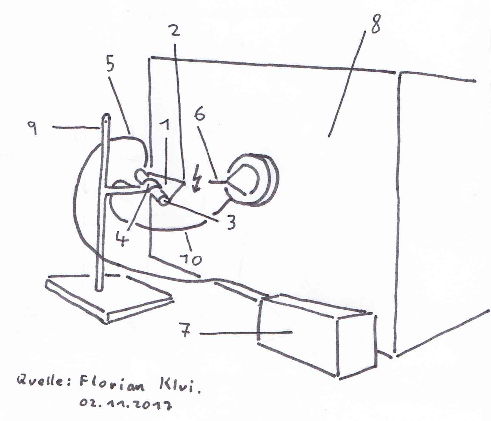
\includegraphics[scale=0.5]{figures/Kapitel4/VWA_MSLeafspray_Versuchsaufbau.png}
  \caption[MS Leafspray Versuchsaufbau, Quelle: Autor]{Leafspray Versuchsaufbau: 1) Filterpapierdreick, 2) Spitze des Dreiecks, 3) Blattmaterial, von Filterpapier umschlossen, 4) Kupferklemme, 5) Kapillare für \gls{lm}, 6) Einlass des Massenspektrometers (mit der markanten Spitze zwecks Verdeutlichung etwas übertrieben dargestellt), 7) \textit{Syringe Pump} - kontrolliert den \gls{lm}-Fluss durch 5), 8) DESI Massenspektrometer, 9) Stativ, 10) Kabel, mit 4) verbunden - zwischen 4) und 6) liegt eine Spannung   an (3-6 kV - durch Blitz zwischen 2) und 6) symbolisiert)}
  \label{fig:LeafsprayVersuchsaufbau}
\end{figure}

Das zu analysierende Blatt wurde zugeschnitten und in Filterpapier eingerollt. Das Filterpapierdreieck wurde in einer Kupferklemme eingespannt (Kapitel \ref{sec:Versuchsdurchfuehrung}). Die Kupferklemme wurde mit einem Kabel (10), das an einem DESI-Massenspektrometer (8) angeschlossen war, verbunden. Zwischen der Kupferklemme (4) und dem Massenspektrometer wurde eine Spannung von 3-6 kV angelegt. Da das Filterpapier mit \gls{lm} benetzt ist und eine Verbindung der Flüssigkeit zur Kupferklemme besteht, kommt es zu einer durch die Spannung ausgelösten Bewegung der im \gls{lm} gelösten Ionen, die nun in das Massenspektrometer hineinfliegen. Der Abstand zwischen Filterpapier (2) und Einlass des Massenspektrometers (6) betrug ungefähr 0.5 cm und ist damit der Flugstrecke der Ionen in natürlicher Umgebung gleichzusetzen. 

\begin{figure}[htbp]
  \begin{subfigure}[b]{0.5\textwidth}
    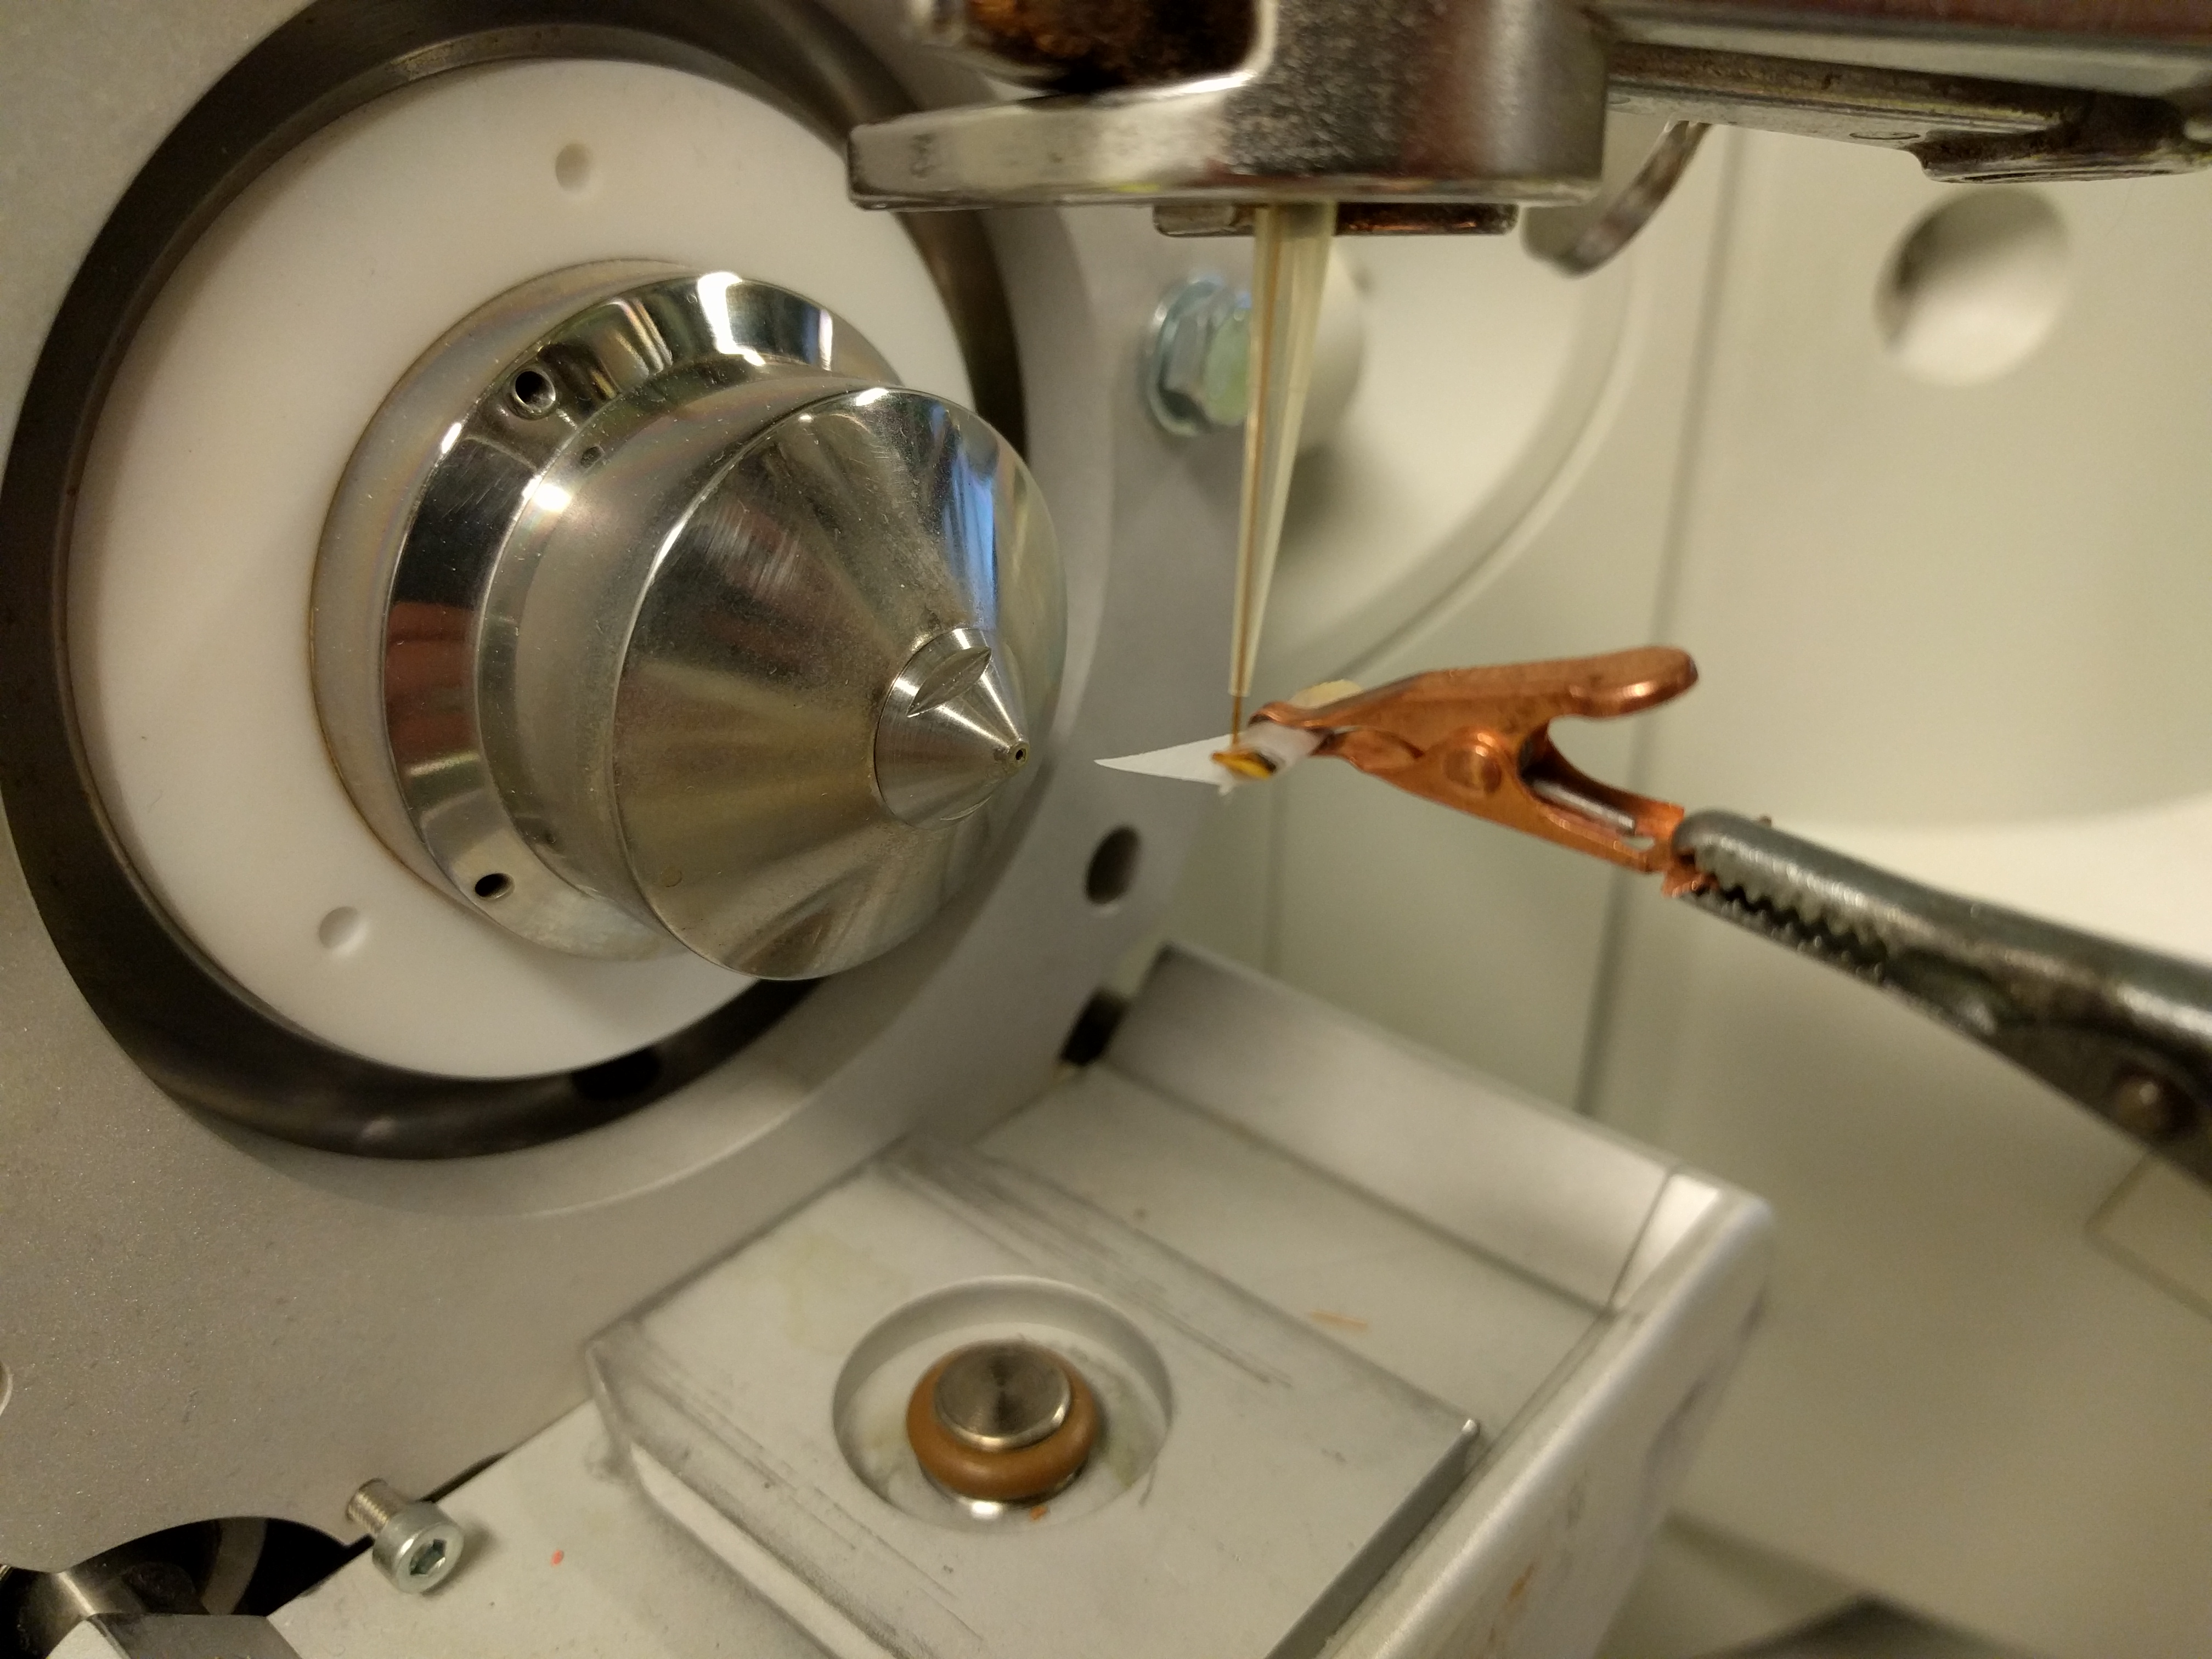
\includegraphics[width=\textwidth]{figures/Kapitel4/VWA_MSLeafspray_Detail1.jpg}
    \caption{}
    \label{fig:MSLeafsprayDetail1}
  \end{subfigure}
  \hfill
  \begin{subfigure}[b]{0.5\textwidth}
    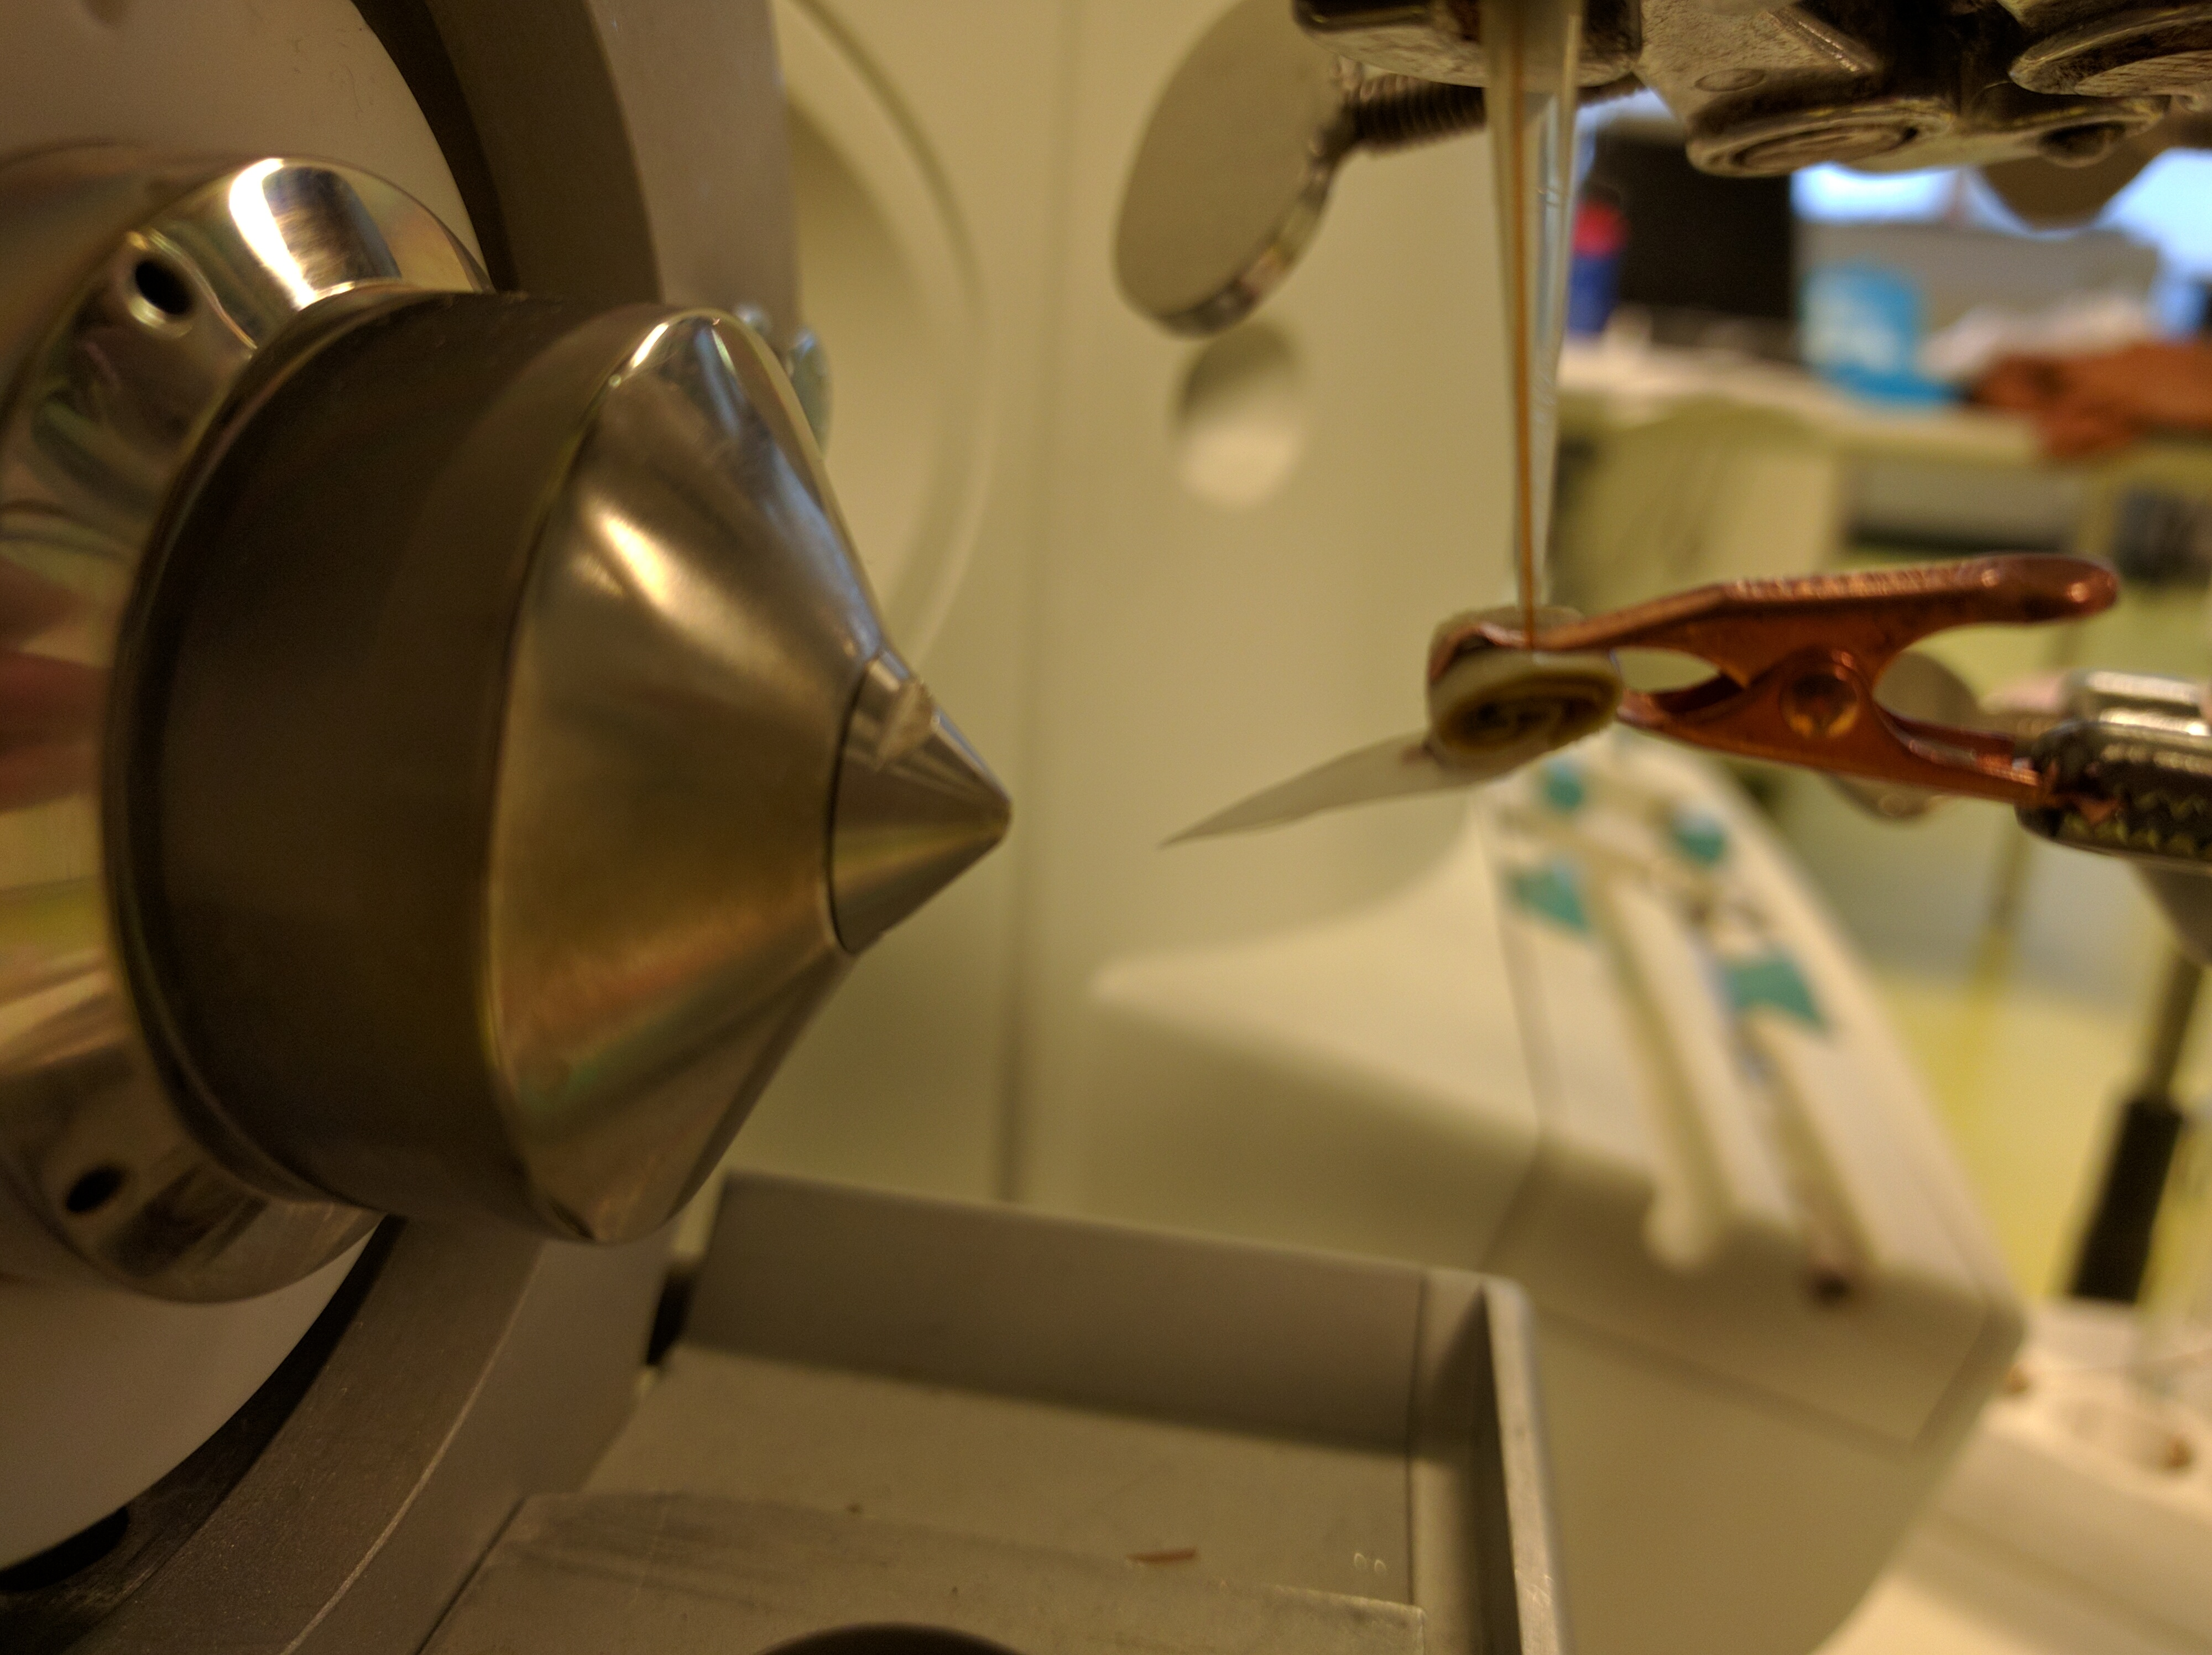
\includegraphics[width=\textwidth]{figures/Kapitel4/VWA_MSLeafspray_Detail2.jpg}
    \caption{}
    \label{fig:MSLeafsprayDetail2}
  \end{subfigure}
  \caption[MS Leafspray Versuchsaufbau Detailfotos, Quelle: Autor]{(a) Einlass des Massenspektrometers mit Kapillare (5), Kupferklemme (4) und Filterpapier mit Blattmaterial (1) und (3), (b) Detailansicht}
  \label{fig:MSLeafsprayDetail}
\end{figure}

In Abbildung \ref{fig:MSLeafsprayDetail} wird gezeigt, wie diese Anordnung umgesetzt wurde. Zu sehen sind die Kupferklemme mit dem eingespannten Filterpapier und dem darin enthaltenen Blatt, die \gls{lm}-Kapillare, die Einlassöffnung des Massenspektrometers und der Abstand von Filterpapierdreicksspitze zum Massenspektrometer. Es gilt zu beachten, dass das Filterpapier in einem gewissen Winkel eingespannt wurde (Abbildung \ref{fig:MSLeafsprayDetail2}), um zu verhindern, dass das \gls{lm} nicht abfließt, was bei einer waagrechten Anordnung in Form einer \textit{Sackbildung} des LM auftreten kann.

\pagebreak
\section{Versuchsdurchführung} \label{sec:Versuchsdurchfuehrung}

Frische, seneszente Brokkoliblätter und Filterpapier wurden mit Rasierklinge und Schere wie in Abbildung \ref{fig:LeafsprayVorbereitung}a ersichtlich zugeschnitten. Anschließend wurde das Brokkoliblatt auf das Filterpapier gelegt und dieses bis zur Basis des Dreiecks eingerollt. 

Diese Art der Vorbereitung zeigte sich als besonders effektiv, da mit ihr höhere Intensitäten der Signale im Massenspektrometer erreicht werden konnten, wie wenn nur das Blatt zu einem Dreieck zugeschnitten und in dieser Form vor das Massenspektrometer gehalten wird. Grund dafür ist vermutlich, dass das \gls{lm} mehr Zeit hat, die Chlorophyllkataboliten aus dem Blatt heraus zu lösen und dass mehr Blattmaterial vorhanden ist. Außerdem behält das Filterpapier länger seine Steifigkeit wie ein Brokkoliblatt, weswegen längere Analysen mit konstanterem Signal möglich sind.

\begin{figure}[hbtp]
  \centering
  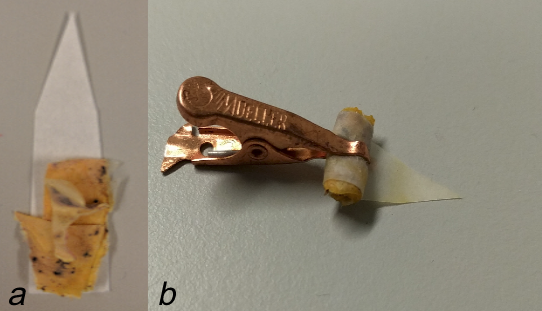
\includegraphics[scale=0.5]{figures/Kapitel4/VWA_MSLeafspray_Blattvobereitung_zwei.png}
  \caption[MS Leafspray Blattvorbereitung, Quelle: Autor]{MS Leafspray Blattvorbereitung: (a) zugeschnittenes Filterpapierdreieck, mit frischen, seneszenten Brokkoliblättern, (b) eingerolltes \textit{Päckchen}, in Kuperklemme eingespannt}
  \label{fig:LeafsprayVorbereitung}
\end{figure}

Das erhaltene \textit{Päckchen} wurde durch eine Kupferklemme (Abbildung \ref{fig:LeafsprayVorbereitung}b) ca. 0.5 cm  vor die Öffnung des Massenspektrometers gehalten (Abbildung \ref{fig:MSLeafsprayDetail2}). Um ein konstantes Signal zu erhalten versorgte eine Kapillare, die wie in Abbildung \ref{fig:MSLeafsprayDetail1} befestigt war, das Päckchen mit einem konstanten \gls{lm}-Fluss (als \gls{lm} wurden \gls{meoh} sowie Acetonitril verwendet). Die Flussrate des \gls{lm} betrug zu Beginn 12 \si{\uL\per\minute}, um das Blatt schneller zu befeuchten und wurde ab dem Erhalt des ersten Signals auf 5 \si{\uL\per\minute} zurückgefahren. Es zeigte sich, dass bei dieser Flussrate das Signal bei annähernd gleichbleibend hoher Intensität am längsten bleibt. Der Spraystrom betrug zwischen xx und xx \si{\micro\ampere}. Diese Geräteeinstellungen sowie Aufarbeitungsmethoden ermöglichten das Messen der Fragmentierungsdiagramme, da hierfür lange Analysezeiten vonnöten sind. Das erste Signal konnte ca. eine Minute nach dem Einschalten der Spannung gemessen werden und erlaubte sinnvolle Messungen bis zu 25 min. \\

\textit{(Platz für Beschreibung der Einstellungen des Gerätes)}\\

Aufgenommen wurden die Massenspektren im Bereich von 300 \gls{mz} bis 1000 \gls{mz}, um  Massenspektren zu bekommen, die nicht so stark von anderen Ionensorten gestört werden. Gemessen wurde im positiven Ionenmodus, wobei zwischendurch in den negativen Ionenmodus geschaltet wurde, wenn die Intensität des Signals im positiven Ionenmodus abnahm. Das Wechseln des Modus konnte die gewünschte Intensität wieder erhöhen. Es wurde somit ein ähnliches Verhalten der Intensitäten im Zeitverlauf beobachtet wie in \cite{RapidScreeningLeafSpray} bereits beschrieben, wobei hier das Umschalten in den negativen Ionenmodus nicht explizit erwähnt wird, um das Problem der abnehmenden Intensitäten im positiven Ionenmodus zu beheben.

\section{Chlorophyllkataboliten des Brokkoliblattes}

Im Folgenden werden die Chlorophyllkataboliten beschrieben, die sich durch MS Leafspray identifizieren ließen. Die Strukturvorschläge wurden durch hochauflösende Massenspektrometrie überprüft. Sie beruhen auf den exakten Molekülmassen und den daraus errechneten möglichen Summenformeln.

Fragmentierungsdiagramme wurden wie in \ref{sec:fragmentierungsdiagramme} beschrieben, erstellt.

\subsection{Bo-NCC-1}

Beim Bo-NCC-1 handelt es sich um einen strukturidenten Kataboliten, wie er auch in der Brokkolifrucht gefunden wurde. \cite{ChlorophyllCatabolitesBroccoli} Gefunden wurde die protonierte Verbindung bei m/z = 793 [M+H]\textsuperscript{+} und das Kaliumsalz bei m/z = 831 [M+K]\textsuperscript{+}. Aufgrund der geringen Intensitäten der protonierten Verbindung war es nicht möglich, ein verwertbares Massenspektrum dieser aufzunehmen. 

Der Katabolit bei m/z = 831 [M+K]\textsuperscript{+} zeigt Abspaltungen von \ch{H2O} bei m/z = 813 [M - \ch{H2O} + K]\textsuperscript{+}, von \ch{CO2} bei m/z = 787 [M - \ch{CO2} + K]\textsuperscript{+} und eine Folge von Abspaltungen bei m/z = 311 [M - (Ring A, Ring D, Zucker, \ch{CO2}) + K]\textsuperscript{+}, bei der Ring A mit dem Zucker, Ring D sowie \ch{CO2} abgespalten wird (siehe Kapitel, Katabolit 619, hochauflösende Massenspektrometrie). Die Abspaltungen bei m/z = 798 [M - (\gls{nAb}) + K]\textsuperscript{+}, m/z = 586 [M - (\gls{nAb}) + K]\textsuperscript{+} und m/z = 551 [M - (\gls{nAb}) + K]\textsuperscript{+} können nicht eindeutig zugeordnet werden, da hierzu weitere experimentelle Daten vonnöten sind. Das Fragment bei m/z = 798 [M - (\gls{meoh}?) + K]\textsuperscript{+} ist insofern interessant, da es sich hierbei um eine Abspaltung von \gls{meoh} (-32 Da) handeln könnte (es wird angenommen, dass die Abweichung um eins durch Ungenauigkeiten des Massenspektrometers zustandekommt), was aber nicht mit der Struktur des Bo-NCC-1 (siehe Abbildung \ref{fig:831MKLeafspraystructure}) vereinbar ist. Aufgrunde ihrer Ungeklärtheit wird auf diese Abspaltung in den weiteren Ausführungen nicht näher eingegangen.

\begin{figure}[htbp]
  
  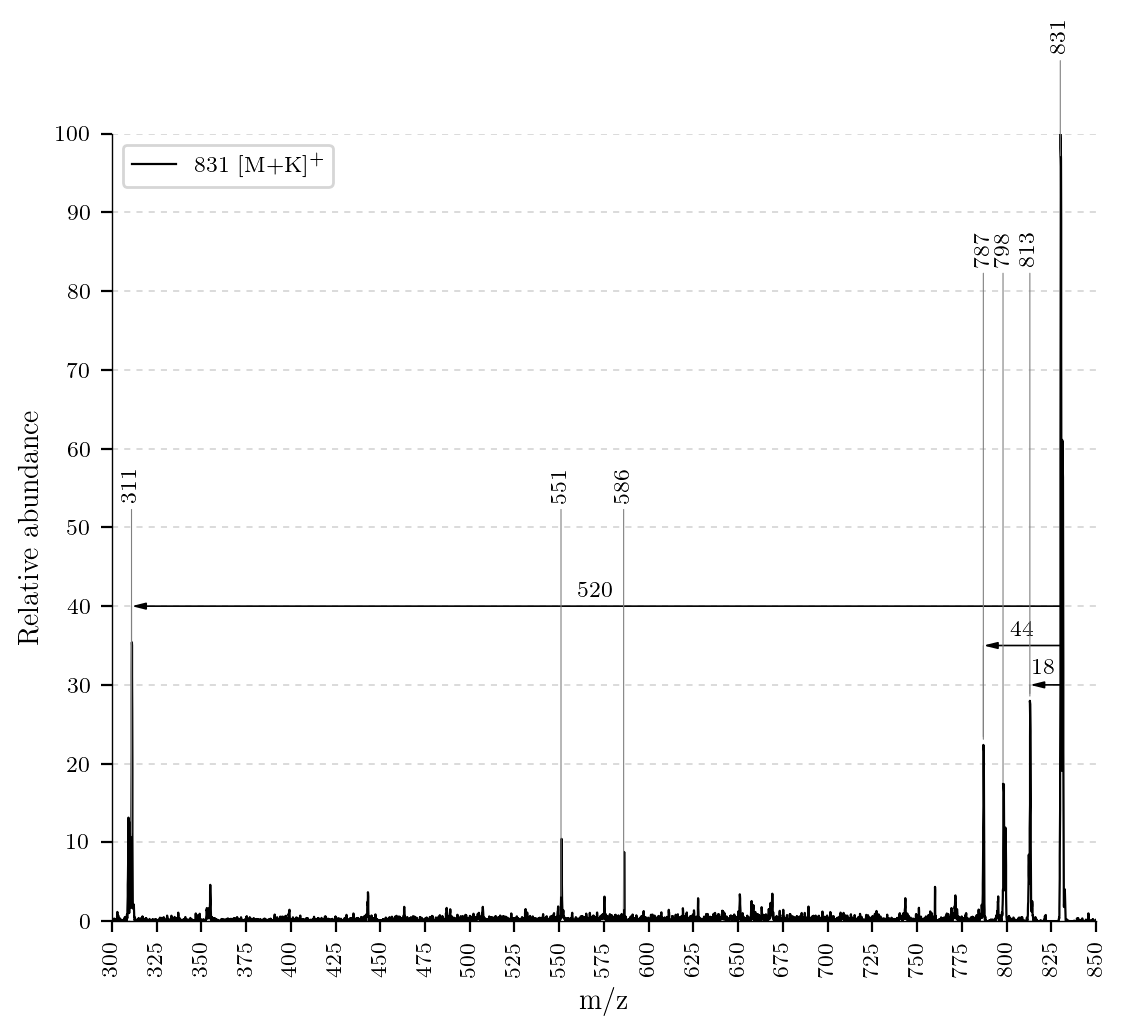
\includegraphics[width=\textwidth, height=0.7\textwidth]{figures/Kapitel4/Kataboliten/VWA_MS_LeafSpray_831.png}
  \label{fig:831MKLeafspray}
  
  \caption[ESI-MS Spektrum von Bo-NCC-1, Quelle: Author]{ESI-MS von Bo-NCC-1 mit m/z = 831 [M+K]\textsuperscript{+}}
\end{figure}

Wie aus dem Fragmentierungsdiagramm (Abbildung \ref{fig:831MKLeafspraydiags}) ersichtlich, erfolgt die Abspaltung von \ch{H2O} bei niedrigeren Energie wie jene von \ch{CO2} und verschwindet bei höheren Energien, wohingegen die Abspaltung von \ch{CO2} erhalten bleibt. Die Abspaltung von \ch{H2O} erreicht ein lokales Maximum bei einer \gls{nKE} von 10. Die Abspaltung erreicht ein lokales Maximum bei 30 \gls{nKE}.

Aufgrund der \ch{CO2} Abspaltung wird an Position .. eine Carbonsäuregrupper vermutet (wie in \cite{StructureElucidation} gezeigt), die über einen Mechanismus wie in Abbildung .. vorgeschlagen, abgespalten wird. Die relativ große Molekülmasse weist auf einen Zucker an Position .. hin. Die Summenformel des Bo-NCC-1 konnte über die exakte Molekülmasse mit einem hochauflösenden Massenspektrometer bestimmt werden.

\begin{figure}[htbp]
  \begin{subfigure}[b]{0.5\textwidth}
    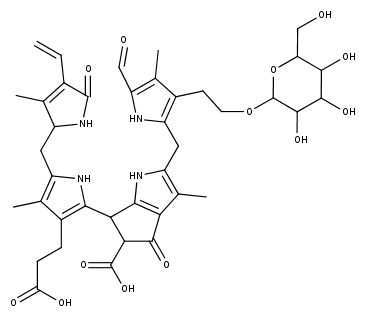
\includegraphics[width=\textwidth]{figures/Kapitel4/Kataboliten/fragmentation_structures/VWA_Katabolit_831.png}
    \caption{}
    \label{fig:831MKLeafspraystructure}
  \end{subfigure}
  \hfill
  \begin{subfigure}[b]{0.5\textwidth}
    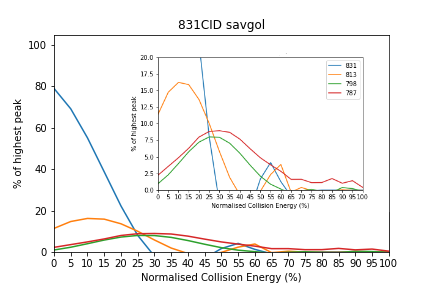
\includegraphics[width=\textwidth]{figures/Kapitel4/Kataboliten/diags/831CID-savgol.png}
    \caption{}
    \label{fig:831MKLeafspraydiags}
  \end{subfigure}
  \caption[Strukturvorschlag von Bo-NCC-1 und Fragmentierungsdiagramm, Quelle: Author]{(a) Strukturvorschlag des Bo-NCC-1 mit Summenformel \ch{C40H48N4O13}, (b) Fragmentierungsdiagramm von Bo-NCC-1 (blau = 831 [M+K]\textsuperscript{+}, orange = 813 [M - \ch{H2O} + K]\textsuperscript{+}, grün = 798 [M - (\ch{MeOH} - \gls{nAb}) + K]\textsuperscript{+}, rot = 787 [M - \ch{CO2} + K]\textsuperscript{+})}
\end{figure}



\subsection{Bo-NCC-3}

Beim Bo-NCC-3 handelt es sich um einen Kataboliten, der nicht in der Brokkolifrucht identifiziert wurde, weswegen er als dritter, in der Brokkolipflanze gefundener Katabolit den Index 3 erhält. \cite{ChlorophyllCatabolitesBroccoli} Analysiert wurde das Kaliumsalz mit m/z = 685 [M+K]\textsuperscript{+}. 

Es wurden zwei charakteristische Abspaltungen von \ch{H2O} bei m/z = 667 [M - \ch{H2O} + K]\textsuperscript{+} sowie von \ch{CO2} bei m/z = 641 [M - \ch{CO2} + K]\textsuperscript{+} beobachtet. Bei den Abspaltungen bei m/z = 429 [M - (\gls{nAb}) + K]\textsuperscript{+}, m/z = 561 [M - (\gls{nAb}) + K]\textsuperscript{+}, m/z = 605 [M - (\gls{nAb}) + K]\textsuperscript{+} und m/z = 652 [M - (\gls{nAb}) + K]\textsuperscript{+} ist nicht eindeutig geklärt, welche Fragmente hierbei entstanden sind. Für das Fragment bei m/z = 652 [M - (\gls{meoh}?) + K]\textsuperscript{+} gilt das gleiche wie bei der Abspaltung von m/z = 798 [M - (\ch{MeOH}?) + K]\textsuperscript{+} von Bo-NCC-1. Um diese Fragmente aufzuklären müssten weitere Experimente des Kaliumsalzes mit einem hochauflösenden Massenspektrometer durchgeführt werden. Fragmentierungen der protonierten Verbindung konnten mit einem hochauflösenden Massenspektrometer identifiziert werden.

\begin{figure}[htbp]
  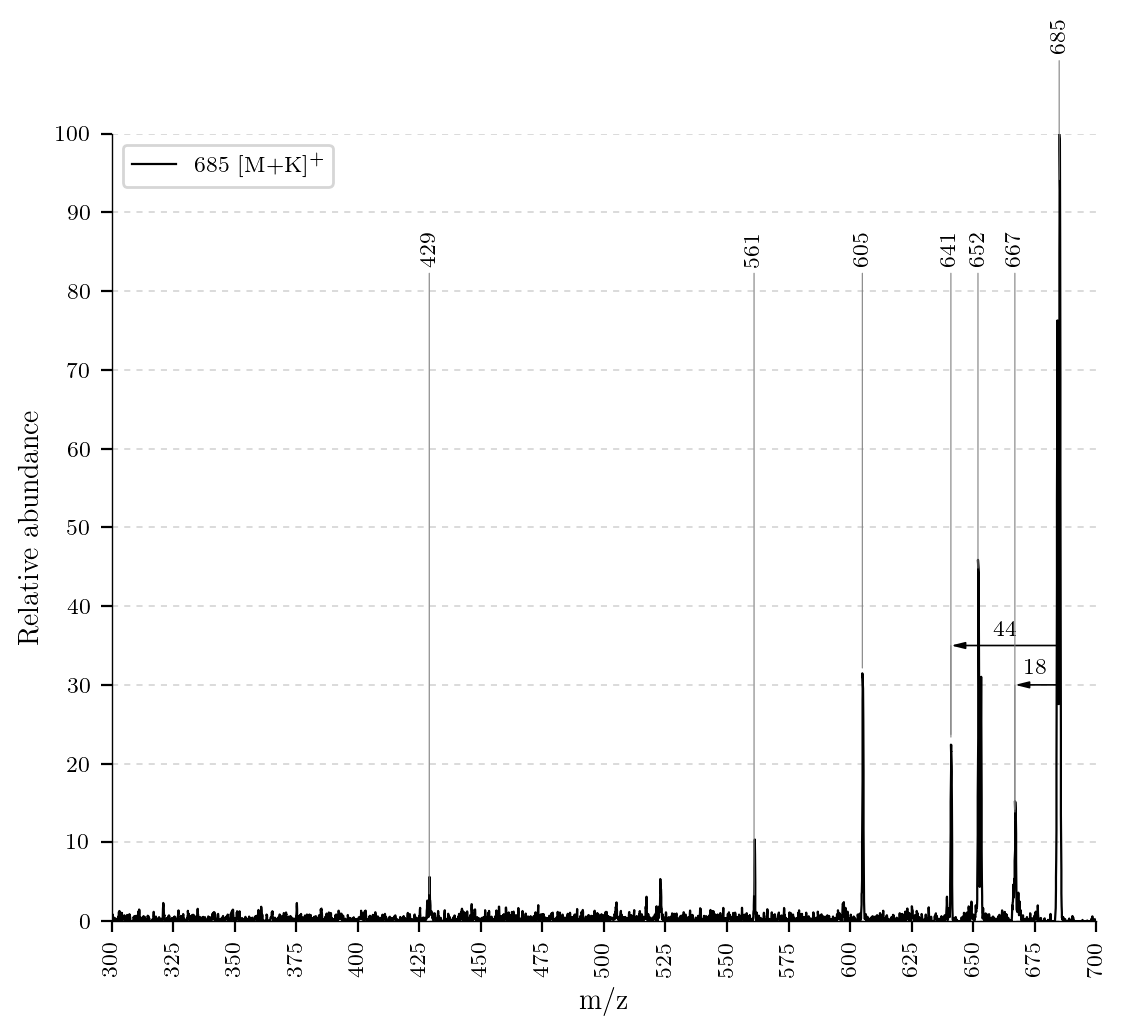
\includegraphics[width=\textwidth, height=0.5\textwidth]{figures/Kapitel4/Kataboliten/VWA_MS_LeafSpray_685.png}
  \label{fig:685MKLeafspray}
  
  \caption[ESI-MS von Bo-NCC-3, Quelle: Author]{ESI-MS von Bo-NCC-3 mit m/z = 685 [M+K]\textsuperscript{+}}
\end{figure}

\begin{figure}[htbp]
  \begin{subfigure}[b]{0.5\textwidth}
    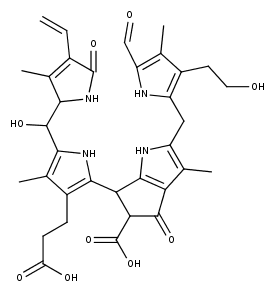
\includegraphics[width=\textwidth]{figures/Kapitel4/Kataboliten/fragmentation_structures/VWA_Katabolit_685.png}
    \caption{}
    \label{fig:685MKLeafspraystructure}
  \end{subfigure}
  \hfill
  \begin{subfigure}[b]{0.5\textwidth}
    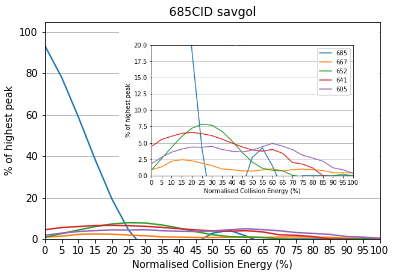
\includegraphics[width=\textwidth]{figures/Kapitel4/Kataboliten/diags/685CID-savgol.png}
    \caption{}
    \label{fig:685MKLeafspraydiags}
  \end{subfigure}
  \caption[Strukturvorschlag von Bo-NCC-3 und Fragmentierungsdiagramm, Quelle: Author]{(a) Strukturvorschlag von Bo-NCC-3 mit Summenformel \ch{C34H38N4O9}, (b) Fragmentierungsdiagramm von Bo-NCC-3 (blau = 685 [M+K]\textsuperscript{+}, orange = 667 [M - \ch{H2O} + K]\textsuperscript{+}, grün = 652 [M - (\gls{meoh}?) + K]\textsuperscript{+}, rot = 641 [M - \ch{CO2} + K]\textsuperscript{+}, violett = 605 [M - (\gls{nAb}) + K]\textsuperscript{+})}
\end{figure}

Das Fragmentierungsdiagramm zeigt, dass die Abspaltung von \ch{H2O} bei einer niedrigeren \gls{nKE} erfolgt, wie jene von \ch{CO2}, da sie ihre höchste Intensität zuvor erreicht (\gls{nKE} von 15 im Vergleich zu 20 von \ch{CO2}). Im Vergleich zum Bo-NCC-1 hat der Graph ein lokales Maximum der \ch{H2O} Abspaltung bei höheren Energien (beim Bo-NCC-3 bei 15 \gls{nKE} - beim Bo-NCC-1 bereits bei 10 \gls{nKE}). Das lokale Maximum der \ch{CO2} Abspaltung verschiebt sich von 30 \gls{nKE} beim Bo-NCC-1 auf 20 \gls{nKE} beim Bo-NCC-3 (Abbildungen \ref{fig:831MKLeafspraydiags} und \ref{fig:685MKLeafspraydiags}). Die potentiellen Abspaltungen von \gls{meoh} bei m/z = 652 [M - (\gls{nAb}) + K]\textsuperscript{+} und bei m/z = 605 [M - (\gls{nAb}) + K]\textsuperscript{+} werden nicht in diese Betrachtungen mit aufgenommen, da ihre Sinnhaftigkeit nicht geklärt ist.

Wie beim Bo-NCC-1 weist die \ch{CO2} Abspaltung auf eine freie Carbonsäure an Position .. hin. Aufgrund der durch die Summenformel erhaltene Sauerstoffanzahl wird angenommen, dass sich an Position .. eine Hydroxygruppe befindet (Abbildung \ref{fig:685MKLeafspraystructure}). Es wird vermutet, dass es sich dabei um eine Vorstuffe zu einem \gls{YCC} handelt. [Referenz]

\subsection{Bo-DNCC}

Es wird vermutet, dass der Bo-DNCC des Brokkoliblattes ident ist mit dem Bo-DNCC der Brokkolifrucht. \cite{ChlorophyllCatabolitesBroccoli} Beobachtet wurden zwei Pseudo-Molekulare Ionen. Eines mit m/z = 619 [M+H]\textsuperscript{+} (Abbildung \ref{fig:619MHLeafspray}) und mit m/z = 657 [M+K]\textsuperscript{+} (Abbildung \ref{fig:657MKLeafspray}).


\begin{figure}[htbp]
  \begin{subfigure}[b]{0.5\textwidth}
    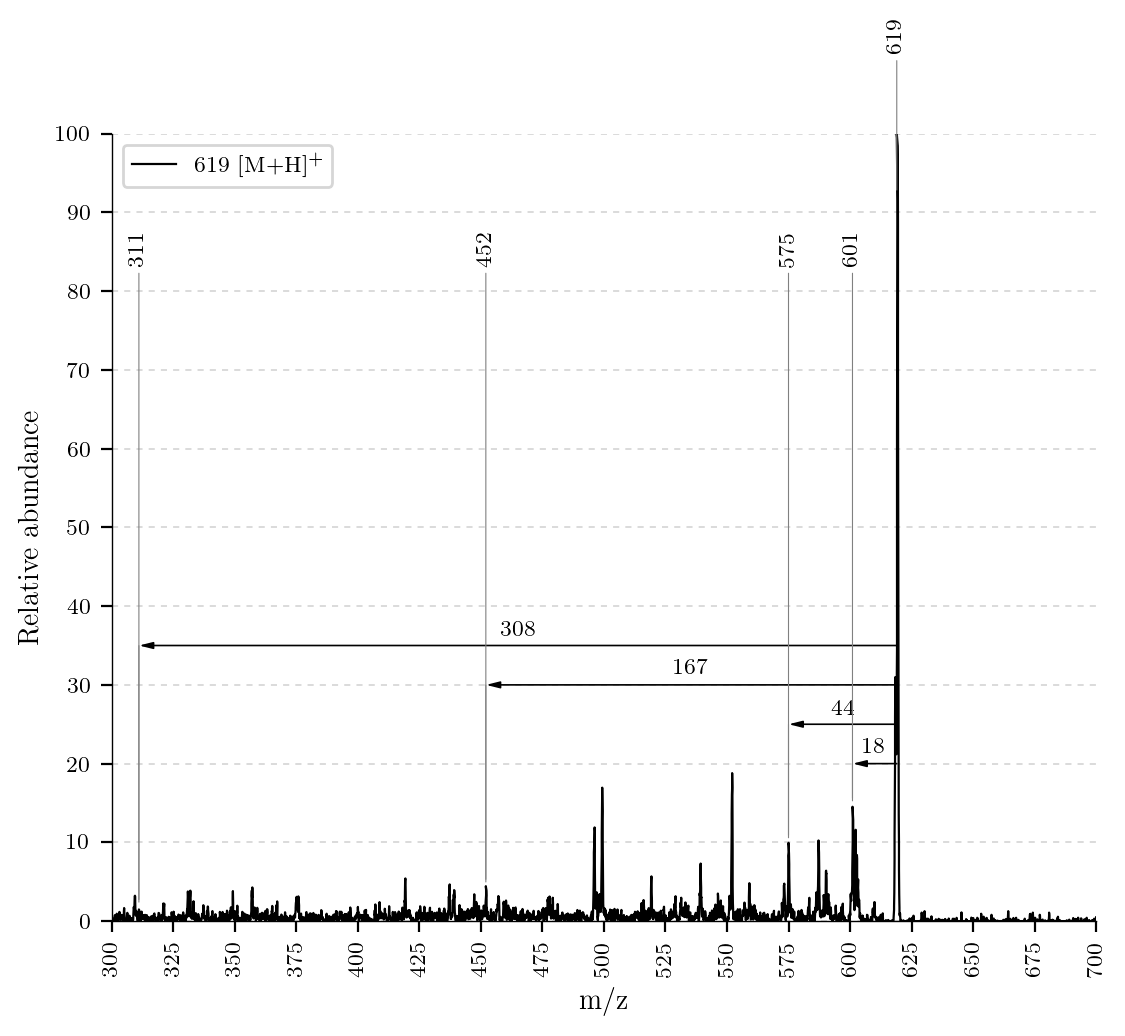
\includegraphics[width=\textwidth]{figures/Kapitel4/Kataboliten/VWA_MS_LeafSpray_619.png}
    \caption{}
    \label{fig:619MHLeafspray}
  \end{subfigure}
  \hfill
  \begin{subfigure}[b]{0.5\textwidth}
    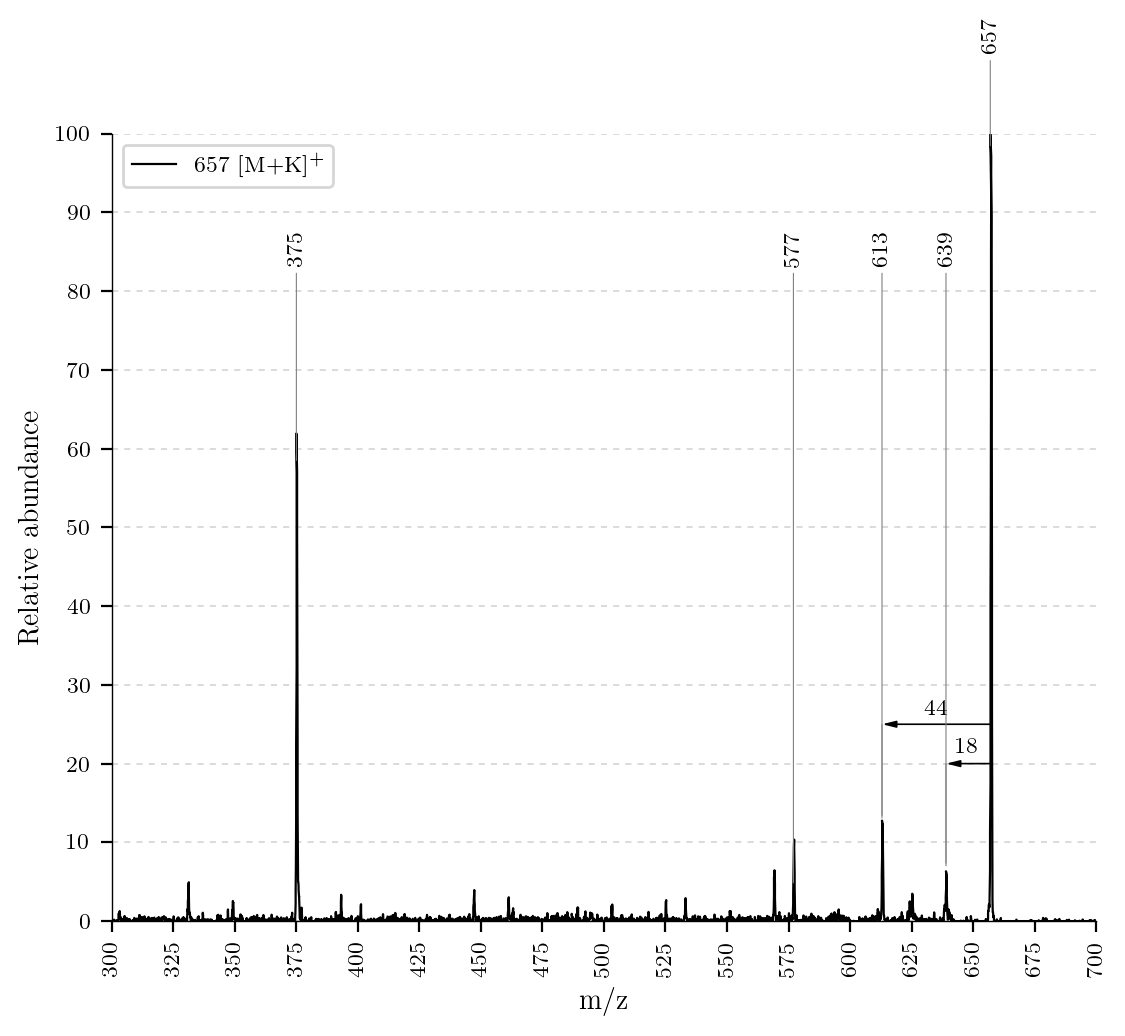
\includegraphics[width=\textwidth]{figures/Kapitel4/Kataboliten/VWA_MS_LeafSpray_657.png}
    \caption{}
    \label{fig:657MKLeafspray}
  \end{subfigure}
  \caption[ESI-MS von Bo-DNCC, Quelle: Author]{ESI-MS von Bo-DNCC: (a) m/z = 619 [M+H]\textsuperscript{+}, (b) m/z = 657 [M+K]\textsuperscript{+}}
\end{figure}


Der Katabolit mit m/z = 619 [M+H]\textsuperscript{+} zeigte Abspaltungen von \ch{H2O} bei m/z = 601 [M - \ch{H2O} + H]\textsuperscript{+}, von \ch{CO2} bei m/z = 575 [M - \ch{H2O} + H]\textsuperscript{+}, von Ring D (zusammen mit einer Abspaltung von \ch{CO2}) bei m/z = 452 [M - (Ring D, \ch{CO2}) + H]\textsuperscript{+} und von Ring A, Ring D und \ch{CO2} bei m/z = 311 [M - (Ring A, Ring D, \ch{CO2}) + H]\textsuperscript{+}.

Das Kaliumsalz des Bo-DNCCs mit m/z = 657 [M+K]\textsuperscript{+} zeigte Abspaltungen von \ch{H2O} bei m/z = 639 [M - \ch{H2O} + K]\textsuperscript{+} und von \ch{CO2} bei m/z = 613 [M - \ch{CO2} + K]\textsuperscript{+}.

\begin{figure}[htbp]
  \begin{subfigure}[b]{0.5\textwidth}
    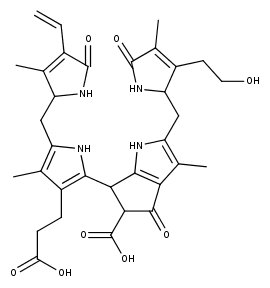
\includegraphics[width=\textwidth]{figures/Kapitel4/Kataboliten/fragmentation_structures/VWA_Katabolit_619.png}
    \caption{}
    \label{fig:619MKLeafspraystructure}
  \end{subfigure}
  \hfill
  \begin{subfigure}[b]{0.5\textwidth}
    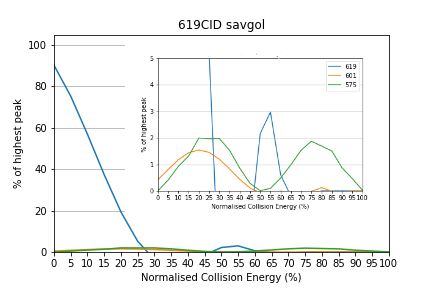
\includegraphics[width=\textwidth]{figures/Kapitel4/Kataboliten/diags/619CID-savgol.png}
    \caption{}
    \label{fig:619MKLeafspraydiags}
  \end{subfigure}
  \caption[Strukturvorschlag von Bo-DNCC mit Fragmentierungsdiagramm, Quelle: Author]{(a) Struktur von Bo-DNCC mit Summenformel \ch{C33H38N4O8}, (b) Fragmentierungsdiagramm von Bo-DNCC (blau = 619 [M+H]\textsuperscript{+}, orange = 601 [M - \ch{H2O} + H]\textsuperscript{+}, grün = 575 [M - \ch{H2O} + H]\textsuperscript{+})}
\end{figure}

 Die \ch{H2O} Abspaltung beim Bo-DNCC erreicht ein lokales Maximum bei 20 \gls{nKE} und erfolgt damit im Vergleich zum Bo-NCC-1 und Bo-NCC-3 bei der höchsten \gls{nKE}. Die Abspaltung von \ch{CO2} weist beim Bo-DNCC zwei lokale Maxima, bei 25 \gls{nKE} und 75 \gls{nKE} auf. Das lokale Maximum an der Stelle 75 \gls{nKE} ist dabei etwas weniger intensiv ausgeprägt wie jenes an der Stelle 25 \gls{nKE}. Das erste lokale Maximum befindet sich damit an der gleichen Stelle wie bei Bo-NCC-1 und Bo-NCC-3 (Abbildungen \ref{fig:831MKLeafspraydiags} und \ref{fig:685MKLeafspraydiags}). Das zweite Maximum kann noch nicht geklärt werden, da es bei den anderen bisher analysierten Kataboliten auch nicht beobachtet wurde.

\section{Identifikation der Reaktionsprodukte} \label{sec:RPMSLeafspray}

Für den Nachweis des Stattfindens der Reaktion der \gls{Chl-K}en mit Essigsäureanhydrid, wurde der gleiche Versuchsaufbau wie in Kapitel \ref{sec:Versuchsaufbau} beschrieben, verwendet. Das Anhydrid als Reaktionsprodukt konnte durch Verwendung von Acetonitril als \gls{lm} isoliert werden. Um eine bessere Identifikation der Reaktionsprodukte zu erreichen, wurden Fragmentierungsdiagramme erstellt.  

\subsection{Reaktionsprodukt von Bo-DNCC}

Das Reaktionsprodukt von Bo-DNCC konnte mit m/z = 699 [M+K]\textsuperscript{+} bestimmt werden (Strukturvorschlag - Abbildung \ref{fig:699MKstructure}). Identifiziert wurde es über die charakteristische Abspaltung von Essigsäure (M = 60 Da) bei m/z = 639 [M - \ch{CH3COOH} + K]\textsuperscript{+}. Ein Mechanismus für die Abspaltung wird in Abbildung \ref{fig:699MKelectronMovement} vorgeschlagen. Dieser Mechanismus ähnelt dem Mechanismus der Abspaltung von \gls{meoh} (\gls{zB} beobachtbar bei einem Cj-NCC), wie in \cite{StructureElucidation} publiziert.\\

\begin{figure}[!htbp]
  \centering
  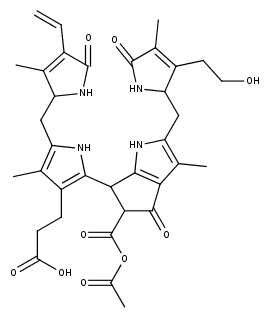
\includegraphics[scale=0.6]{figures/Kapitel4/Kataboliten/fragmentation_structures/VWA_Katabolit_699.png}
  \caption[Strukturvorschlag des Reaktionsproduktes von Bo-DNCC, Quelle: Autor]{Strukturvorschlag des Reaktionsproduktes mit Summenformel \ch{C35H41N4O9}}
  \label{fig:699MKstructure}
\end{figure}

Es wurden Abspaltungen von \ch{H2O} bei m/z = 681 [M - \ch{H2O} + K]\textsuperscript{+}, von \ch{CH3COOH} bei m/z = 639 [M - \ch{CH3COOH} + K]\textsuperscript{+} und von Ring A und Ring D mit \ch{CO2} bei m/z = 311 [M - (Ring A, Ring D, \ch{CO2}) + K]\textsuperscript{+} beobachtet. 

Zur Identifikation der Reaktionsprodukte wurde die \ch{CH3COOH} Abspaltung aufgrund ihrer Dominanz und Eindeutigkeit herangezogen (\gls{uA} Abbildung \ref{fig:699MKstructurediags2}). Das Fragment bei m/z = 599 [M - (\gls{nAb}) + K]\textsuperscript{+} ist interessant, da eine Abspaltung von 100 Da bei anderen Kataboliten ebenfalls beobachtet wurde. Die anderen Fragmentierungen in Abbildung \ref{fig:699MKLeafspray} konnten nicht zugeordnet werden. \\

\begin{figure}[!htbp]
  \centering
  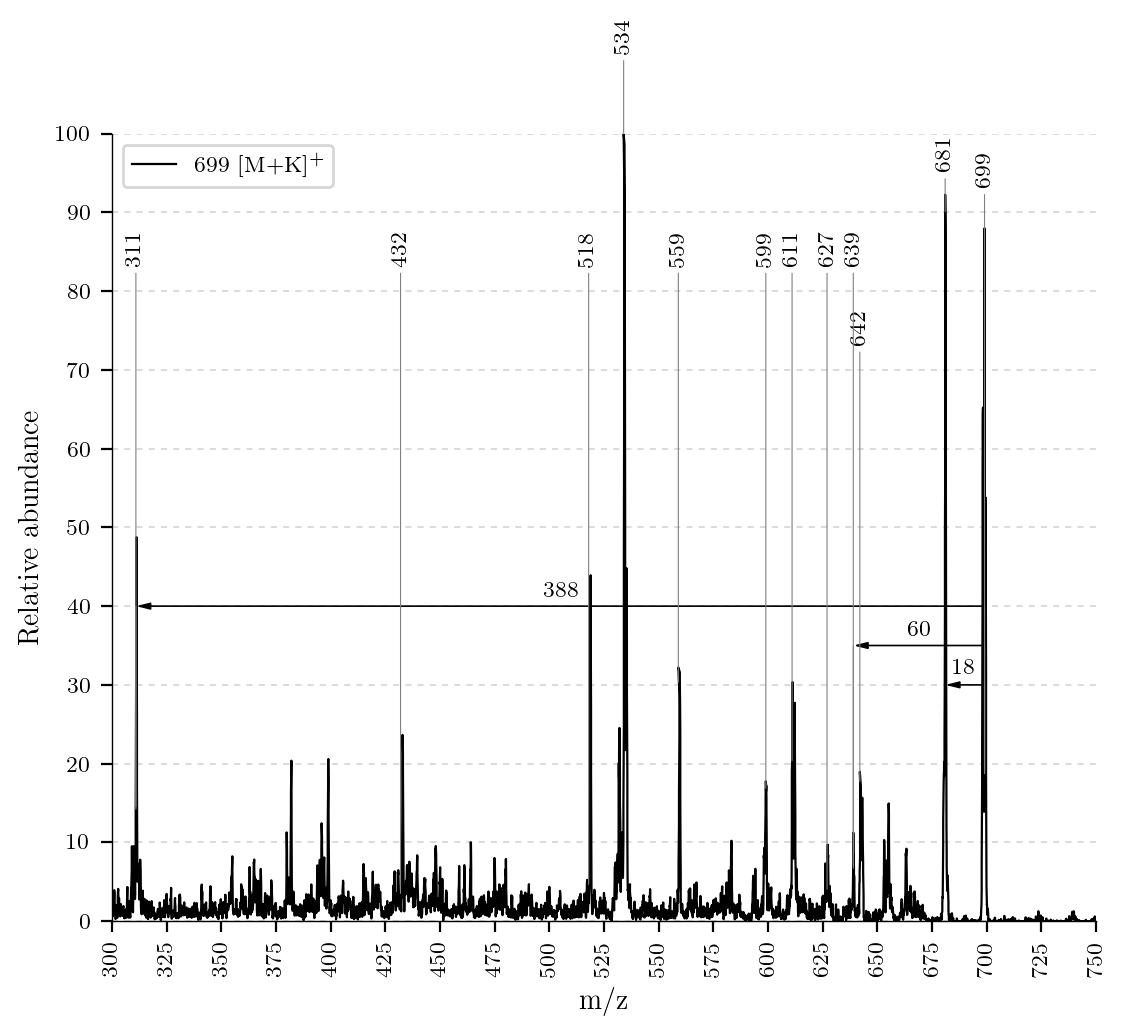
\includegraphics[width=\textwidth, height=0.6\textwidth]{figures/Kapitel4/Kataboliten/VWA_MS_LeafSpray_699.png}
  \caption[ESI-MS Spektrum des Reaktionsproduktes von Bo-DNCC, Quelle: Autor]{ESI-MS Spektrum des Reaktionsproduktes mit m/z = 699 [M+K]\textsuperscript{+}}
  \label{fig:699MKLeafspray}
\end{figure}

Diskussion der Abspaltung bei m/z = 599 [M - (\gls{nAb}) + K]\textsuperscript{+}: Die Abspaltung von 100 Da bei m/z = 599 [M - (\gls{nAb}) + K]\textsuperscript{+} erreicht im Fragmentierungsdiagramm lokale Maxima bei 15 \gls{nKE} und 30 \gls{nKE}. Lokale Minima befinden sich bei 17 \gls{nKE} und 40 \gls{nKE}, an jenen Stellen, an der die Abspaltung von \ch{CH3COOH} lokale Maxima aufweist (Abbildung \ref{fig:699MKstructurediags2}). Daraus könnte man Informationen über den Mechanismus der Abspaltung ableiten. Man könnte sagen, dass die Abspaltung von 100 Da einhergeht mit jener von \ch{CH3COOH} und dass sie mechanistisch miteinander verknüpft sind, also, dass bevor einer Abspaltung des Fragments mit 100 Da \ch{CH3COOH} abgespalten werden muss. Es ließe sich damit erklären, warum bei einem Maximum der einen Abspaltung die andere Abspaltung ein Minimum aufweist.\\ 


\begin{figure}[!htbp]
  \begin{subfigure}[b]{0.5\textwidth}
    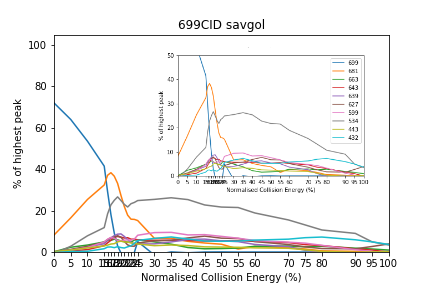
\includegraphics[width=\textwidth, height=\textwidth]{figures/Kapitel4/Kataboliten/diags/699CID-savgol2.png}
    \caption{}
    \label{fig:699MKLeafspraydiags1}
  \end{subfigure}
  \hfill
  \begin{subfigure}[b]{0.5\textwidth}
    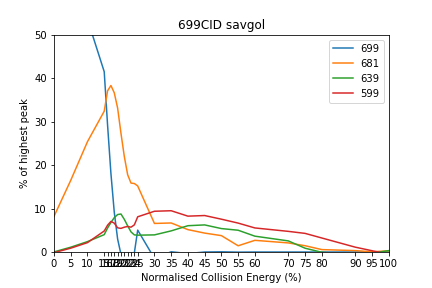
\includegraphics[width=\textwidth, height=\textwidth]{figures/Kapitel4/Kataboliten/diags/699CID-savgol1.png}
    \caption{}
    \label{fig:699MKstructurediags2}
  \end{subfigure}
  
  \caption[Fragmentierungsdiagramme des Reaktionsproduktes von Bo-DNCC, Quelle: Autor]{(a) Fragmentierungsdiagramm des Bo-NCC-3 mit allen beobachteten Abspaltungen (blau = 699 [M+K]\textsuperscript{+}, orange = 681 [M - \ch{H2O} + K]\textsuperscript{+}, grün = 663 [M - (2x\ch{H2O}) + K]\textsuperscript{+}, rot = 643 [M - (\gls{nAb}) + K]\textsuperscript{+}, violett = 639 [M - \ch{CH3COOH} + K]\textsuperscript{+}, braun = 627 [M - (\gls{nAb}) + K]\textsuperscript{+}, pink = 599 [M - (\gls{nAb}) + K]\textsuperscript{+}, grau = 534 [M - (\gls{nAb}) + K]\textsuperscript{+}, hellgrün = 443 [M - (\gls{nAb}) + K]\textsuperscript{+}, türkis = 432 [M - (\gls{nAb}) + K]\textsuperscript{+}), (b) Fragmentierungsdiagramm mit ausgewählten Abspaltungen (blau = 699 [M+K]\textsuperscript{+}, orange = 681 [M - \ch{H2O} + K -\ch{H2O}, grün = 639 [M - \ch{CH3COOH} + K], rot = 599 [M - (\gls{nAb}) + K]\textsuperscript{+})}
\end{figure} 

Im Fragmentierungsdiagramm erreicht die \ch{H2O} Abspaltung ein lokales Maximum bei 17 \gls{nKE}. Die Abspaltung nimmt bis zu 30 \gls{nKE} stark ab und bleibt bis zu 90 \gls{nKE} erhalten. Im Vergleich zum Fragmentierungsdiagramm des nicht reagierten Bo-DNCC erfolgt die \ch{H2O} Abspaltung bei einer niedrigeren \gls{nKE} und ist länger beobachtbar (vergleiche Abbildungen \ref{fig:619MKLeafspraydiags} und \ref{fig:699MKstructurediags2}). Es gilt zu bedenken, dass beim nicht reagierten Bo-DNCC das [M+H]\textsuperscript{+}-Ion aufgenommen wurde, wohingegen man beim reagierten Bo-DNCC das [M+K]\textsuperscript{+}-Ion analysierte. Der Unterschied im Verlauf der Kurven könnte somit auch durch diesen Umstand hervorgerufen werden.

Die Abspaltung von \ch{CH3COOH} besitzt lokale Maxima bei 20 \gls{nKE} und 45 \gls{nKE}. Das Maximum bei 45 \gls{nKE} ist weniger intensiv. Die Intensität der Abspaltung nimmt dabei kontinuierlich bis zu einer von 80 \gls{nKE} ab (Abbildung \ref{fig:699MKstructurediags2}). Ein lokales Minimum der Abspaltung befindet sich zwischen 23 \gls{nKE} und 30 \gls{nKE}. \\



\begin{figure}[!htbp]
  \begin{subfigure}[b]{0.5\textwidth}
    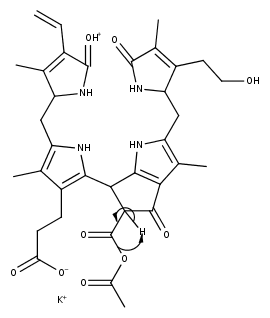
\includegraphics[width=\textwidth, height=\textwidth]{figures/Kapitel4/Kataboliten/fragmentation_structures/VWA_Katabolit_699-639_MK_electronMovement.png}
    \caption{}
    \label{fig:699MKelectronMovement}
  \end{subfigure}
  \hfill
  \begin{subfigure}[b]{0.5\textwidth}
    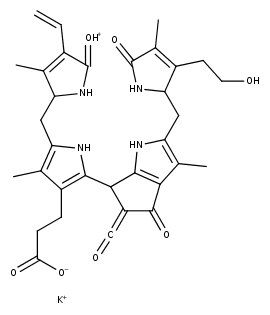
\includegraphics[width=\textwidth, height=\textwidth]{figures/Kapitel4/Kataboliten/fragmentation_structures/VWA_Katabolit_699-639_MK.png}
    \caption{}
    \label{fig:699MK639}
  \end{subfigure}
  \caption[Vorschlag des Mechanismus der \ch{CH3COOH} Abspaltung, Quelle: Autor]{(a) vorgeschlagener Mechanismus der Essigsäureabspaltung und (b) das Produkt, wobei \ch{CH3COOH} als stabiles Neutralteilchen abgespalten wird}
\end{figure}



\pagebreak
\subsection{Reaktionsprodukt von Bo-NCC-3}

Die Molekülmasse des Reaktionsproduktes von Bo-NCC-3 konnte mit m/z = 727 [M+K]\textsuperscript{+} bestimmt werden. Eine Abspaltung von Essigsäure wurde bei m/z = 667 [M+K]\textsuperscript{+} beobachtet. Weiters wurde eine Abspaltung von \ch{H2O} bei m/z = 709 [M - \ch{H2O} + K]\textsuperscript{+} beobachtet. Bei der Abspaltung bei m/z = 627 [M - (\gls{nAb}) + K]\textsuperscript{+} könnte es sich um die gleiche Abspaltung wie beim Reaktionsprodukt des Bo-DNCC handeln, da auch ein Fragment mit M = 100 Da abgespalten wird. Die anderen Abspaltungen (Abbildung \ref{fig:727MKLeafspray}) konnten nicht eindeutig zugeordnet werden.

\begin{figure}[!htbp]
  \centering
  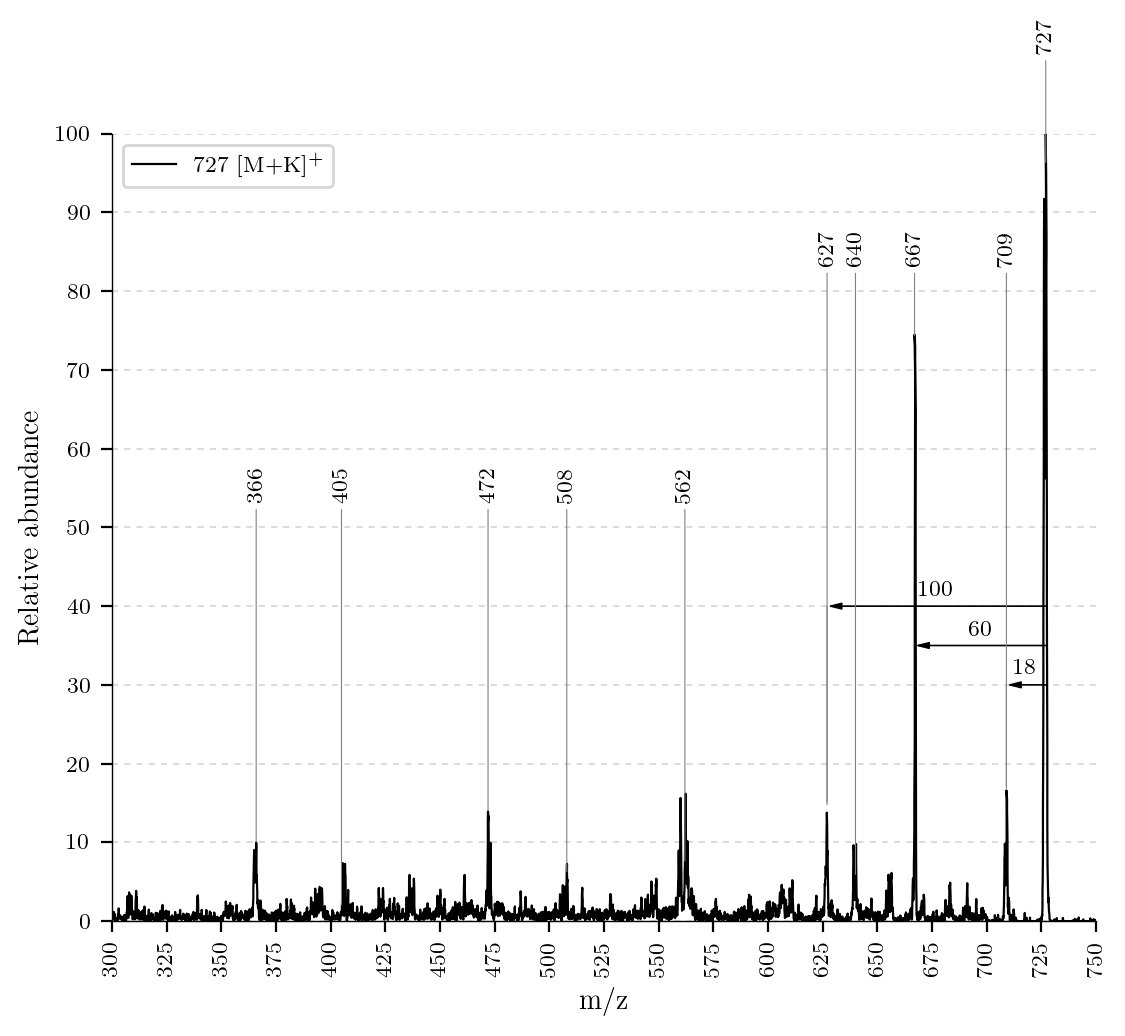
\includegraphics[width=\textwidth, height=0.7\textwidth]{figures/Kapitel4/Kataboliten/VWA_MS_LeafSpray_727.png}
  \caption[ESI-MS des Reaktionsproduktes von Bo-NCC-3, Quelle: Autor]{ESI-MS Spektrum des Reaktionsproduktes bei m/z = 727 [M+K]\textsuperscript{+}}
  \label{fig:727MKLeafspray}
\end{figure}

\begin{figure}[!htbp]
  \centering
  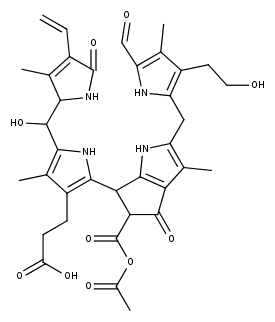
\includegraphics[scale=0.6]{figures/Kapitel4/Kataboliten/fragmentation_structures/VWA_Katabolit_727.png}
  \caption[Strukturvorschlag des Reaktionsproduktes von Bo-NCC-3, Quelle: Autor]{Strukturvorschlag des Reaktionsproduktes mit Summenformel \ch{C36H40N4O10}}
  \label{fig:727MKstructure}
\end{figure}

Es wurde beobachtet, dass die Abspaltung von \ch{H2O} bei niedrigeren Energien erfolgt wie jene von \ch{CH3COOH}. Im Vergleich zum Fragmentierungsdiagramm des Reaktionsproduktes des Bo-DNCC (Abbildung \ref{fig:699MKLeafspraydiags1}) kann als Charakteristikum der \ch{CH3COOH} Abspaltung ein lokales Maximum bei 45 \gls{nKE} gedeutet werden (Abbildung \ref{fig:699MKstructurediags2} und Abbildung \ref{fig:727MKLeafspraydiags}). Die Abspaltung von \ch{H2O} weist bei beiden Kataboliten ein lokales Maximum bei 15 \gls{nKE} auf und besitzt einen ähnlichen Kurvenverlauf (Abbildung \ref{fig:699MKstructurediags2} und Abbildung \ref{fig:727MKLeafspraydiags}). Dies lässt darauf schließen, dass es sich bei dieser \ch{H2O}-Abspaltung um eine Abspaltung auf ein und dersselben Position handelt. Als Position der Abspaltung wird die Hydroxygruppe an Position 32 des Chl-Kataboliten vorgeschlagen. 

\begin{figure}[!htbp]
  \centering
  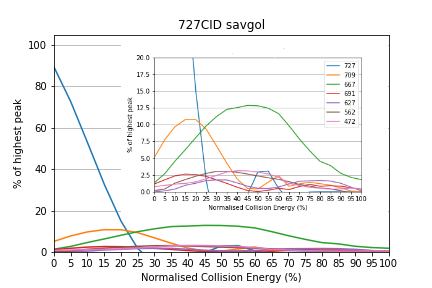
\includegraphics[scale=0.7]{figures/Kapitel4/Kataboliten/diags/727CID-savgol.png}
  \caption[Fragmentierungsdiagramm des Reaktionsproduktes von Bo-DNCC, Quelle: Autor]{Fragmentierungsdiagramm des Reaktionsproduktes (lbau = 727 [M+K]\textsuperscript{+}, orange = 709 [M - \ch{H2O} + K]\textsuperscript{+}, grün = 667 [M - \ch{CH3COOH} + K]\textsuperscript{+}, rot = 691 [M - ? + K]\textsuperscript{+}, violett = 627 [M - ? + K]\textsuperscript{+}, braun = 562 [M - ? + K]\textsuperscript{+}, pink = 472 [M - ? + K]\textsuperscript{+})}
  \label{fig:727MKLeafspraydiags}
\end{figure}



\subsection{Reaktionsprodukt von Bo-NCC-1}

Erwartungsgemäß konnte das Reaktionsprodukt des Bo-NCC-1 bei m/z = 873 [M+K]\textsuperscript{+} gefunden werden. Es zeigt Abspaltungen von \ch{H2O} bei m/z = 855 [M - \ch{H2O} + K]\textsuperscript{+}, von Essigsäure bei m/z = 813 [M - \ch{CH3COOH} + K]\textsuperscript{+}und von \ch{CH3COOH}, Ring A, Ring D, zweimal \gls{meoh} und \ch{CO} bei m/z = 309 [M - (Ring A, Ring D, 2mal MeOH, \ch{CO})  + K]\textsuperscript{+} (diesselbe Abspaltung wurde beim Reaktionsprodukt m/z = 661 [M+H]\textsuperscript{+} beobachtet - Kapitel \ref{sec:ESIMSRPBoNCC3}). Beim Fragment m/z = 441 [M - (Ring D, 2mal MeOH, \ch{H2O}) + K]\textsuperscript{+} könnte es sich um eine Abspaltung von Ring D, zweimal \gls{meoh} und \ch{H2O} handeln. 

\begin{figure}[htbp]
  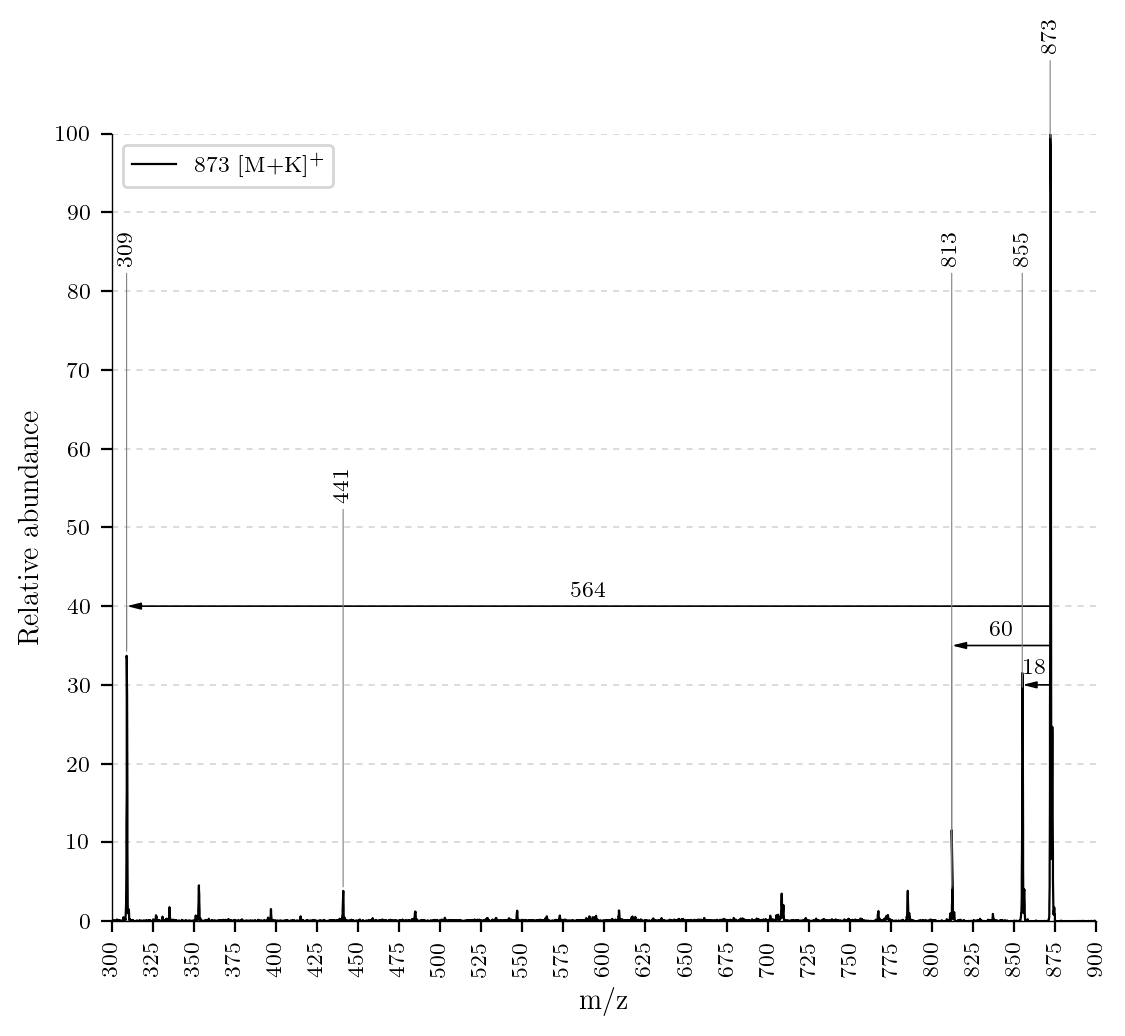
\includegraphics[width=\textwidth, height=0.7\textwidth]{figures/Kapitel4/Kataboliten/VWA_MS_LeafSpray_873.png} 
  \caption[ESI-MS des Reaktionsproduktes von Bo-NCC-1, Quelle: Autor]{ESI-MS des Reaktionsproduktes bei m/z = 873 [M+K]\textsuperscript{+}}
  \label{fig:873MKLeafspray}
\end{figure}

\begin{figure}[htbp]
  \centering
  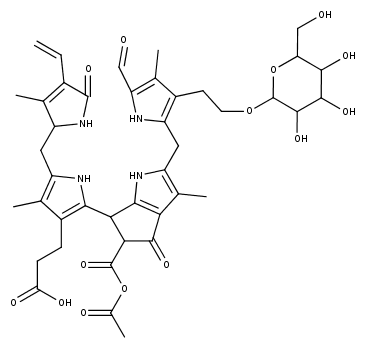
\includegraphics[scale=0.6]{figures/Kapitel4/Kataboliten/fragmentation_structures/VWA_Katabolit_873.png}
  \caption[Strukturvorschlag des Reaktionsproduktes von Bo-NCC-1, Quelle: Autor]{Strukturvorschlag des Reaktionsproduktes mit Summenformel \ch{C42H50N4O14}}
  \label{fig:873MKstructure}
\end{figure}

Im Fragmentierungsdiagramm sieht man, dass sich das lokale Maximum der Essigsäureabspaltung hin zu niedrigeren Energien verschoben hat. Es befindet sich nun bei  35 \gls{nKE}. Auch die \ch{H2O} Abspaltung verschiebt sich zu niedrigeren Energien und besitzt ein lokales Maximum bei 10 \gls{nKE}. Im Vergleich zum Bo-DNCC und Bo-NCC-3 nahmen diese Werte um 10 bzw. 5 Einheiten an \gls{nKE} ab. Dieser Zusammenhang wurde in zwei voneinander unabhängigen Experimenten beobachtet (Abbildung \ref{fig:873MKLeafspraydiags1} und Abbildung \ref{fig:873MKstructurediags2}). Die Ursache könnte beim Zuckerring liegen, der die Elektronenverteilung vermutlich so beeinflusst, dass die Abspaltungen bereits bei niedrigeren Energien erfolgen. 

(Einfügen von 3D Bildern, die die sterischen Zusammenhänge vorschlagen).

\begin{figure}[!htbp]
  \begin{subfigure}[b]{0.5\textwidth}
    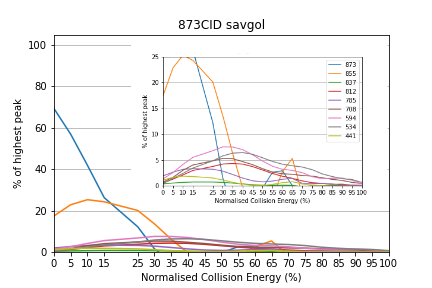
\includegraphics[width=\textwidth, height=\textwidth]{figures/Kapitel4/Kataboliten/diags/873CID-savgol1.png}
    \caption{}
    \label{fig:873MKLeafspraydiags1}
  \end{subfigure}
  \hfill
  \begin{subfigure}[b]{0.5\textwidth}
    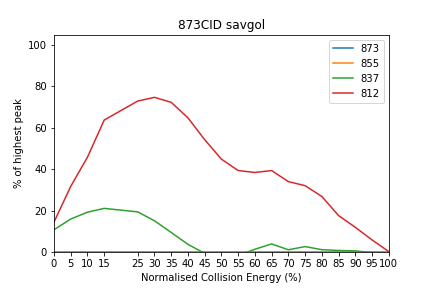
\includegraphics[width=\textwidth, height=\textwidth]{figures/Kapitel4/Kataboliten/diags/873CID-savgol2.png}
    \caption{}
    \label{fig:873MKstructurediags2}
  \end{subfigure}
  
  \caption[Fragmentierungsdiagramm des Reaktionsproduktes von Bo-NCC-1, Quelle: Autor]{Fragmentierungsdiagramm des Reaktionsproduktes: (a) Experiment am 13.09.2017 (11:00) - (blau = 873, orange = 855, grün = 837, rot = 812, violett = 765, braun = 708, pink = 594, grau = 534, hellgrün = 441), (b) Experiment am 13.09.2017 (09:45) - schlechter gelungen, weswegen die Abspaltungen nicht so schön wie in Experiment (a) zu sehen sind (blau = 873, orange = 855, grün = 837, rot = 812}
\end{figure}